\documentclass[tikz,border=2pt]{standalone}
\usepackage{amsmath}
\usetikzlibrary{arrows.meta}
\begin{document}
% Number in system L(t) = A(t) - D(t) for A = (1,2,5,9,10), D = (4,6,7,11,13) (single server):
% L = Q + L_s with L_s(t) = 1 on [1,7) and [9,13) (red layer), Q(t) = 1 on [2,4), [5,6), [10,11) (blue layer).
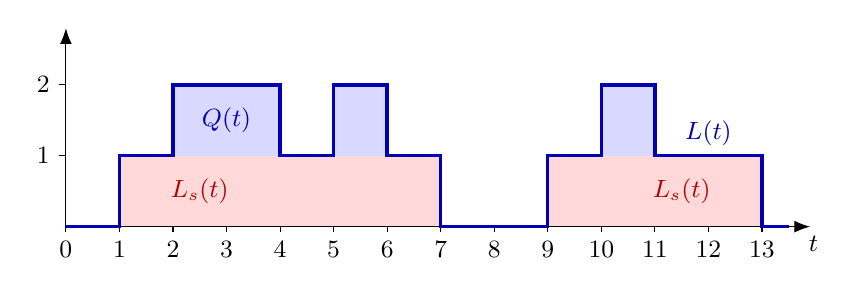
\begin{tikzpicture}[font=\small, >={Latex[length=2mm]}, x=0.68cm, y=0.9cm]
  % layers
  \fill[red!15] (1,0) rectangle (7,1);
  \fill[red!15] (9,0) rectangle (13,1);
  \foreach \a/\b in {2/4, 5/6, 10/11} \fill[blue!15] (\a,1) rectangle (\b,2);
  \node[red!70!black] at (2.5,0.5) {$L_s(t)$};
  \node[red!70!black] at (11.5,0.5) {$L_s(t)$};
  \node[blue!70!black] at (3,1.5) {$Q(t)$};
  % axes
  \draw[->] (0,0) -- (13.9,0) node[anchor=north west, xshift=-4pt] {$t$};
  \draw[->] (0,0) -- (0,2.8);
  \foreach \t in {0,1,...,13} \draw (\t,0) -- (\t,-0.07) node[below] {$\t$};
  \foreach \n in {1,2} \draw (0,\n) -- (-0.12,\n) node[left] {$\n$};
  % number in system
  \draw[blue!70!black, very thick] (0,0) -- (1,0) -- (1,1) -- (2,1) -- (2,2) -- (4,2) -- (4,1) -- (5,1)
    -- (5,2) -- (6,2) -- (6,1) -- (7,1) -- (7,0) -- (9,0) -- (9,1) -- (10,1) -- (10,2) -- (11,2)
    -- (11,1) -- (13,1) -- (13,0) -- (13.5,0);
  \node[blue!70!black, anchor=south] at (12,1) {$L(t)$};
\end{tikzpicture}
\end{document}
